%!TEX root = ../thesis.tex

\section{Systemic functional linguistics} \label{sect:sfl}

\Glsxtrfull{SFL} is a functional\hyp{}semantic theory of language and context, used throughout this thesis as a theoretical framework for conceptualising and understanding \emph{texts}. The central focus of the theory is the \gls{SFG}, which guides the investigation presented in Chapters \ref{chap:introdata}--\ref{chap:experiential}, and which is used to link \glslink{lexicogrammar}{lexicogrammatical} choices found in \gls{Forum} contributions to \gls{discourse-semantic} meanings in Chapter \ref{chap:discuss-bp}.

As a theory of language, \gls{SFL} can be understood as centrally concerned with three axes:

\begin{enumerate}
\item A \textbf{cline of instantiation}, with language as a system at one end, and individual texts (i.e. realisations) of the system at the other
\item A \textbf{hierarchy of stratification}, where contexts have probabilistic effects on the meaning, content and expression in a text
\item An \textbf{array of metafunctions} that language is structured to accomplish (role-relationship negotiation, the construal of experience, and self-organisation of text into coherent units)
\end{enumerate}
%
The theory has evolved from the early work of Michael Halliday \parencite*[e.g.][]{halliday_1966_deepgrammar,halliday1978language}, with substantial further contributions from \textcite[e.g.][]{hasan_structure_1985}, Martin \parencite*[e.g.][]{martin_english_1992} and Matthiessen \parencite*[e.g.][]{matthiessen_lexicogrammatical_1995}. That said, much of the theory's conceptualisation of language can be traced to developments in linguistics in the first half of the 20th century. In the sections below, I elaborate on the three axes identified above, situating each within a brief historical context.

\subsection{Cline of instantiation}

The cline of instantiation is the space between the linguistic system and an actual sample of real-language use. The cline invokes the Saussurean distinction between language and speech \parencite*{saussure_course_1916}, but rather than treating each as conceptually different, positions each as occupying a pole on an axis of \emph{instantiation}. \gls{SFL} also expands upon the Saussurean position, by considering language not as a study of signs, but of \emph{sign-systems}---`not sets of individual things, but rather networks of relationships' \cite[p.~4]{halliday_language_1989}. In between the two poles are \glslink{lexicogrammar}{lexicogrammatical} systems of increasing delicacy, which extend from broad grammatical choices (between indicative and non\hyp{}indicative Mood, for example) toward and up to lexis. In this way, \gls{SFL} treats lexis and grammar as two ends of the same stratum. \gls{SFL} presents this axis in the form of \emph{system networks}, which represent speakers' possible choices and their constraints on more delicate selections. Doing text analysis in \gls{SFL} therefore chiefly involves relating text (an instance) to the overall meaning potential of the system.

\subsection{Hierarchical structure of language and context}

In \gls{SFL}, language and context are organised hierarchically as \emph{strata}, with every stratum realised through the stratum below. Following the anthropological work of Malinowski, context is divided into two strata: a \emph{cultural dimension}, which shapes all interactions taking place within the culture, and a \emph{situational dimension}, which concerns the specific environment in which a given text is produced \cite[p.~6]{halliday_language_1989}. Following Hjelmslev (e.g. 1946), language is also stratified into register, semantics, \gls{lexicogrammar} and phonology\slash graphology (depending on whether or not the text is spoken\slash written).

Within the \glslink{lexicogrammar}{lexicogrammatical} stratum, we can observe a more detailed kind of hierarchical order, the \emph{rank scale} (Table \ref{tab:rankscale}). The nature of the hierarchy is different, however: in the stratification of language and context, each stratum \emph{realises} the stratum above; in the rank scale, each level is comprised by one or more instances of the rank(s) below. \nocite{halliday_concept_1966}

%todo: reference around here
\begin{table}[ht]
\centering
\begin{tabular}{l}

\toprule
Clause complex       \\
Clause               \\
Group\slash phrase   \\
Word                 \\
Morpheme             \\
\bottomrule
\end{tabular}
\caption[Rank Scale]{Rank Scale (Halliday, 1966)}
\label{tab:rankscale}
\end{table}
%
\noindent Incongruent realisation, or \emph{grammatical metaphor}, expands the meaning potential of language \cite{heyvaert_nominalization_2003}: through this device, realisations of one rank through another (for example) may be chosen by speakers to satisfy experiential, interpersonal or textual goals. These realisations are typically \emph{agnate} (that is, closely related) in terms of experiential semantics \cite{matthiessen_key_2010}.

%Moving down the scale from system, the meaning potential of the language as a whole becomes progressively narrowed, beginning with genres and registers, and narrowing further with text types, until we arrive at an individual text (an instance of language) \cite{martin_genre_2006}

%In \gls{SFL}, language users are seen as making choices at the level macro strata that place constraints on what can be realised at lower strata \cite{martin_genre_2006}. After a choice of semantic meaning is made, for example, the speaker is presented with congruent and incongruent realisations of the semantic meaning within the lexicogrammar. Incongruent realisation, or \emph{grammatical metaphor}, is the mechanism by which language can have limitless meaning potential \cite{heyvaert_nominalization_2003}: through this device, `atypical' realisations of one rank through another (for example) may be chosen by speakers to satisfy experiential, interpersonal or textual goals. Politeness, for example, may be achieved by incongruent Mood and Modality seletions.

\subsection{Metafunctions of language}

The final major dimension of \gls{SFL} is the division between metafunctions of language. In \gls{SFL}, language users are seen as simultaneously attending to three metafunctions, each of which is responsible for making a different kind of meaning. Each of the metafunctions is realised concurrently by distinct \glslink{lexicogrammar}{lexicogrammatical} systems. The \emph{interpersonal metafunction}, realised by the \sctext{Mood} and \sctext{Modality} systems, conveys and negotiates role-relationships between interlocutors. The \emph{experiential metafunction},\endnote{In Hallidayan \gls{SFL}, experiential meanings and logical meanings together comprise the experiential metafunction. In the vein of \textcite{eggins_introduction_2004}, this thesis discusses only experiential meaning, and all references to the transitivity system concern only experiential function.} realised by the system of \sctext{Transitivity}, is used by speakers to construe doings and happenings in the real world, inner states of consciousness, and relationships between things and events. The \emph{textual metafunction},\endnote{Despite their potential relevance as a means of explicating the ways in which turn-taking is operationalised in \glspl{OSG}, textual meanings are not covered in significant detail here due to limitations in scope.} realised by the system of \sctext{\gls{THEME}} creates coherence within and between texts \cite{eggins_introduction_2004}.

%Each function is operationalised at the \glslink{lexicogrammar}{lexicogrammatical} level of language, and as such, can be captured by the grammar.

% not analysed in the case study, is responsible for the reflexive organisation of units of language into coherent texts.

%These social functions are divided into three kinds of meaning: \textbf{interpersonal meanings}, which construct and negotiate role-relationships between speakers; \textbf{experiential meanings}, which communicate doings and happenings in the world; and \textbf{textual meanings}, which reflexively organise language into coherent, meaningful sequences. Through the hiearchy of stratification, \gls{discourse-semantic} functions are each realised in speakers' \glslink{lexicogrammar}{lexicogrammatical} choices by different grammatical systems. In Englsh, interpersonal meanings are made via the Mood and Modality systems. Experiential meanings are made through the Transitivity system. Textual meanings are made through referential and conjunctive functions, as well as the system of Theme and Rheme (see Figure \ref{fig:eggins}).

\begin{figure}[htb]
\centering
\addvbuffer[12pt 8pt]{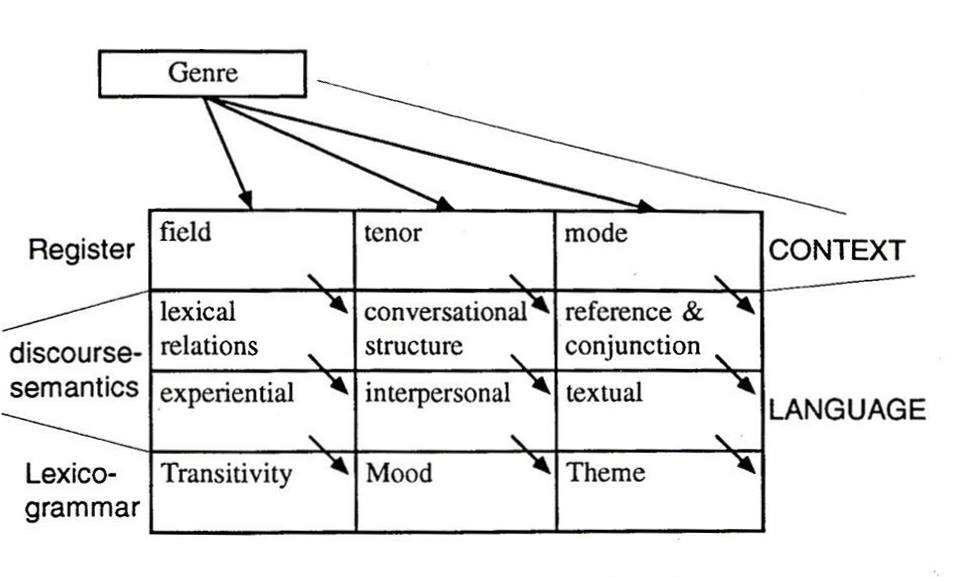
\includegraphics[width=0.65\textwidth]{../images/egginsfixed.jpg}}
\caption[Strata and metafunctions of language]{Strata and metafunctions of language (adapted from Eggins, 2004)}
\label{fig:eggins}
\end{figure}

\subsection{Affordances of \glsfmtshort{SFL} for researching an \glsfmtshort{OSG}}

\gls{SFL} has been applied to a diverse array of research areas including first and second language acquisition \cite{halliday1993towards,hasan_learning_1994}, language pedagogy \cite{halliday_towards_1993}, historical linguistics \cite{cummings2010introduction,martin_re/reading_2003} and (critical) discourse analysis \cite{hunston_systemic_2013,le_systematic_2009,martin_working_2003}. For the latter of these, \gls{SFL} is particularly useful, and has for this reason become one of the most popular grammars and theories of language for discursive research: as Halliday explains, at the most general level, \gls{SFL} is used `to understand the quality of texts: why a text means what it does, and why it is valued as it is' \parencite*[p.~xxx]{halliday_introduction:_2004}. In fact, from a systemic\hyp{}functional perspective, the use of a grammar is a prerequisite for all discourse analytic research. In Halliday's words,

\begin{quote}\small\singlespacing
it is sometimes assumed that discourse analysis, or `text linguistics' can be carried on without grammar---or even that it is somehow an alternative to grammar. But this is an illusion. A discourse analysis that is not based on grammar is not an analysis at all, but simply a running commentary on a text \parencite*[p.~xvii]{halliday_introduction:_2004}).
\end{quote}
%
%todo: reword again?
As a result of this conviction, the organisation and metalanguage of \gls{SFL} has in part been designed with text analysis in mind.

%todo: add zappavigna , hunston, cmc contexts...

The overall utility of \gls{SFL} for analysis of an \gls{OSG} may be divided into three main factors: the treatment of language as constitutive of text, the notion of language as a meaning\hyp{}making resource, and the division of interpersonal and experiential metafunctions within a grammar. These three factors are outlined below.

\subsubsection{Language as constitutive of context} \label{sect:context-in-text}

Though context is an increasingly central concern within many branches of linguistics, \gls{SFL} is notable for the extent to which its theory of context has been articulated and empirically applied \cite{widdowson_text_2008}. Halliday explains that in \gls{SFL}, context and text are in fact seen as `aspects of the same process', and that any sample of language use thus in fact `goes beyond what is said and written: it includes [...] the total environment in which a text unfolds' \parencite*[p.~5]{halliday_language_1989}. Therefore, \gls{SFL} treats language as constitutive of, rather than simply bound to, its context. As context can often be accurately deduced from text alone, and as context can be used to predict appropriate kinds of texts, some \gls{SFL} theorists contend that \emph{context is in text} \cite[e.g.][p.~7]{eggins_introduction_2004}. Context and language thus together construct both a reality and roles for people within it \cite{veel_learning_1997}.

This notion of language as simultaneously constructing and responding to the demands of contexts of situation has often formed an implicit theoretical assumption in online community and \gls{OSG} research: many works reviewed in the previous chapter tacitly take the perspective that language \emph{must} be responsible for the development of distinct cultures in online groups, as language is often the sole semiotic system available to group members \cite{thorne_computer-mediated_2008}.

%The absence of research explicitly drawing upon \gls{SFL} for online discourse socialisation research is thus striking.

\subsubsection{Language as a meaning-making resource}

The \glslink{SFL}{systemic\hyp{}functional} approach foremost involves an understanding of language as a semiotic system strategically drawn upon by language users as a meaning\hyp{}making resource---`how people use language with each other in accomplishing everyday social life' \cite[p.~2]{eggins_introduction_2004}. The orientation of the theory toward function and meaning\hyp{}making may be contrasted with phrase structure grammars, which typically do not attempt to account for meaning or pragmatics, and which are not grounded in analysis of realised linguistic patterns, but instead seek to provide rules that conform to speakers' intuitions regarding what is grammatically possible to say \cite{martin_english_1992}. \gls{SFL}, in contrast, understands language as \emph{purposive}: its use is motivated by purposes that may or may not be transparent or tangible. This is an appropriate theoretical stance for investigations of linguistic choices in an online community, because all communities are inherently social, and because in text\hyp{}based \gls{CMC} language is the main resource upon which members can draw to achieve their respective goals.

%\paragraph{Quantifiability of linguistic features}
%Halliday explains that it is possible to evaluate texts by counting the frequencies of relevant phenomena...
%Halliday remarks on the potential usefulness of very large datasets \parencite*{halliday_language_1992}
%This is amenable to the corpus-based approach taken here.

\subsubsection{Interpersonal and experiential functions of language}

%todo: add a ref to harvey so it doesn't seem like a fudge
From a systemic perspective, the simultaneous provision of health information and social support within \glspl{OSG} is realised by \glslink{member}{users} attending simultaneously to two metafunctions of language: an interpersonal dimension, responsible for negotiating role relationships, and an experiential dimension, responsible for communicating propositions about the world. This is the most useful affordance of \gls{SFL} for investigation of \glspl{OSG}, because the division of types of meaning is central to the reason for the community's existence: if the social element were not desired, \glslink{member}{users} would likely be content to simply read from static pages; if experiential content were not desired, health communities and the threads within them would not need to be organised by topic and subtopic. The interest in the phenomenon of \emph{advice} noted in Section \ref{sect:advice} would likewise stand to benefit from clearer delineation of the relationship between social roles and ideational content, each of which occupies a distinct, but overlapping space within acts of advising or directing others to act. Such a delineation would likely not be unwelcome. Early conceptualisations of the process of social support bear striking resemblance to the systemic model of interpersonal meaning: \textcite[p.~11]{shumaker1984toward} remind us, for instance, that social support is foremost `an exchange of resources between two individuals'.

\subsubsection{\glsfmtshort{SFL} and corpus linguistics}

In systemic\hyp{}functional terms, the \gls{corpus} is a large collection of instances of language use. These instances are typically organised by register, or by register dimensions. Automated counting of patterns in these instances is one possible way to uncover the grammar---that is, the patterns that generalise across the instances. A particular benefit of \gls{CL} approaches is that they make it possible to sketch out the probabilities of certain choices in certain contexts. At the same time, \gls{CL} approaches can test key tenets of \gls{SFL} theory \cite{honnibal_creating_2007}. \textcite{clarke_patterns_2012}, for example, uses a corpus-based approach to test the context metafunction hookup hypothesis---that is, the connection between language and context.

\gls{CL} and \gls{SFL} also share a number of underlying similarities. Most obviously, both are concerned with analysis of natural language, and both share a conceptualisation of \emph{register} as playing a significant role in shaping the \glslink{lexicogrammar}{lexicogrammatical} patterns to be found within texts \cite{hunston_systemic_2013}. Another key point of convergence between \gls{SFL} and \gls{CL} is in the treatment (explicit in \gls{SFL}, generally implicit in \gls{CL}) of context as being \emph{contained within} instantiated texts---`context is in text', rather than around it \cite{eggins_introduction_2004}. Systemicists evidence this assertion through the fact that we can often accurately deduce the overall functions, purposes and genres of highly decontextualised fragments of texts: \emph{Submissions must contain 8--10 references} can be quickly identified as part of a set of instructions for the submission of academic work, based purely on its lexical (submissions, references) and grammatical (nominalisation, modalisation, etc.) properties. In the same way, Halliday conceptualises \glslink{lexicogrammar}{lexicogrammatical} features of texts as probabilistically determined by their context. That is to say, a given constellation of interpersonal, experiential and textual variables (e.g. the writing of a professor to undergraduates in a written course overview) will likely contain the kinds of \glslink{lexicogrammar}{lexicogrammatical} features described in the example above \cite{halliday_corpus_1991}. This conceptualisation is of great benefit to corpus linguists interested in discourse analysis: given that \gls{CL} methods inherently involve the stripping of contextual information from natural language, and that analysis of contextualised language is preferred within the discourse analytic tradition, the recognition of context within \gls{lexicogrammar} allows \gls{CL} practitioners to address the common claim  \cite[e.g.][]{virtanen_discourse_2009} that \glslink{CL}{corpus} and discourse linguistic approaches, having very different orientations toward context, are difficult to reconcile.

\subsection{Overview of relevant elements of \glsfmtshort{SFG}}

%ntodo: sfl glossary weirdness
The core of \gls{SFL} is its grammar, known as the \glsxtrfull{SFG}, which is organised along the three axes discussed above. In this section, I describe the parts of the \gls{SFG} that are most relevant to the case study. The major references for this section include \citeauthor{halliday_introduction_2004} 2004, \citeauthor{matthiessen_lexicogrammatical_1995} 1995, and \citeauthor{eggins_introduction_2004} 2004.

\subsubsection{Register}

%todo: clean up, no repeating
Register occupies the level of abstraction above \glspl{discourse-semantic}, where language interfaces with a context of situation. The total content of each metafunction (interpersonal, experiential and textual) respectively corresponds to the three register variables of \emph{Tenor}, \emph{Field} and \emph{Mode} \cite{halliday_language_1989}. Halliday provides a minimal definition of each component:

\begin{enumerate}
\item  `The \sctext{Field of discourse} refers \emph{to what is happening}'
\item `The \sctext{Tenor of discourse} refers to \emph{who is taking part}'
\item `The \sctext{Mode of discourse} refers to \emph{what part the language is playing}' \parencite*[p.~12]{halliday_language_1989}
\end{enumerate}
%
In \gls{SFL}, doing register analysis can refer either to creating qualitative descriptions of the Field, Tenor and \gls{Mode} of a text (or collection of related texts), or to the process of generating quantitative, corpus\hyp{}based models of these features \cite{lukin2011halliday,matthiessen_modeling_2015}. Qualitative descriptions are intended to provide `[an interpretation of] the social context of a text, the environment in which meanings are being exchanged' \cite[p.~12]{halliday_language_1989}. Quantitatively, the internal dimensions of a single register can be modelled by counting relevant \glslink{lexicogrammar}{lexicogrammatical} features. The distribution of Process Types and the participants engaged in them, for instance, can be used to determine how speakers construe the world around them; \sctext{Mood} features can be analysed in order to see how speakers position themselves with respect to others (see below). 

Using a cartographic metaphor, \textcite{matthiessen_modeling_2015,Matthiessen2015} calls for further work within functional linguistics that models the internal dimensions of registers, and then situates these models within a cluster of related registers (presented later as Figure \ref{fig:pie-of-fortune}). By comparing these distributions to those found in other registers, registers can be arranged as a landscape, either along the axis of stratification or instantiation. The ultimate, perhaps distant goal, is to synthesise information about individual registers, in order to form a description of the meaning potential of a language, realising the notion of language as `an assembly or assemblage of registers' \parencite*[p.~44]{matthiessen_modeling_2015}. 

\textcite{matthiessen_applying_2013} has also applied register analysis to the domain of healthcare. Within the \gls{consumercentred} paradigm, this means focussing on individual healthcare consumers' health journeys, rather than on, for example, how consumers move through a given hospital or clinic in general. These healthcare journeys, Matthiessen explains, consist of sequence of encounters with formal and informal healthcare institutions. Each encounter presents a registerial configuration of topic, interactants and media: we may speak with a doctor in a busy clinic about our symptoms, or to a mental health practitioner about our personal relationships in an hour\hyp{}long consultation; we may phone an insurance carrier to clarify an issue about coverage, and write to a family member on Facebook about what we have learned. The case study of this thesis, centred on the registerial environment of an \gls{OSG}, has yet to be described within \gls{SFL} or \gls{HC} literature. The registerial description provided in Chapter \ref{chap:discuss-bp} is therefore intended to facilitate the addition of this register to the current body of knowledge and descriptions of the kinds of registers that may be encountered within consumers' journeys beyond the clinic.

%These meanings are realisations within the \sctext{Mood} and \sctext{Transitivity} choices that \gls{Forum} \glspl{member} make in their \glspl{post}. The two metafunctions and their implicated grammatical systems are described below. Chapters \ref{chap:researchdesign}--\ref{chap:experiential} combine to provide a quantitative model of the register of the \glslink{Forum}{Bipolar Forum}. Chapter \ref{chap:discuss-bp} presents a qualitative summary of Field, Tenor and Mode.

\subsubsection{Interpersonal meanings, MOOD and MODALITY} \label{sect:mood}

The Tenor variable of register is realised by interpersonal meanings. In turn, these meanings are made via the \sctext{Mood} and \sctext{Modality} systems of the \gls{lexicogrammar}. The interpersonal metafunction is responsible for negotiating role\hyp{}relationships with other speakers. It thus facilitates a constant \emph{exchange} of material and semiotic commodities; it is used to \emph{enact}, and to \emph{interact}.

\paragraph{Speech Function and Mood\slash Indicative Type}

In the \gls{SFG}, at the broadest level, utterances involve two potential \emph{speech roles}: \emph{giving} and \emph{demanding}. Within either speech role, two types of commodities may potentially be given or demanded: \emph{information}, or \emph{goods and services}. This leads to four main \emph{speech functions}, each of which is congruently realised by a different \sctext{Mood Type}. Information is given via statements, which are realised with declarative Mood. Information can be demanded via questions, congruently realised with the interrogative Mood. Goods and services are given via modalised declaratives. Demands for these non\hyp{}semiotic commodities are made via commands, which are realised with (non-indicative) imperative Mood. These intrastratal relationships are summarised in Table \ref{tab:roles}.

\begin{table}[htb]
\centering\small
\begin{tabular}{lll}

\toprule
\textbf{} & \textbf{Information} & \textbf{Goods and services} \\ 
\midrule
\textbf{Giving}   & statement $\rightarrow$ declarative    & offer $\rightarrow$ modalised interrogative     \\ 
\textbf{Demanding}   & question $\rightarrow$ interrogative & command $\rightarrow$ imperative    \\
\bottomrule
\end{tabular}
\caption[Mood Type and Speech Function]{Speech roles, commodities, speech functions and congruent \sctext{Mood Types} in SFL}
\label{tab:roles}
\end{table}   

\paragraph{Grammar of the \sctext{Mood} system} \label{sect:mood-grammar}

Each indicative clause contains a \emph{Mood Block}, comprised of a \emph{Subject} and \emph{Finite}. Optionally, clauses may also contain a \emph{Residue Block}, which can include a \emph{Predicator}, a \emph{Complement}, and\slash or one or more \emph{Adjuncts}. As non-indicatives, imperatives are comprised entirely of the Residue Block. In the case of declaratives, to determine which element is the Mood Block, a reverse-polarity tag can be added to the end of the declarative:

\begin{quote}
Geoff had difficulty with the task, \emph{didn't he?}
\end{quote}
%
Whatever is referenced by the pronoun in the tag is the Subject component of the Mood Block. The Finite is the first verb or modal in the verbal group that follows. It too is duplicated in a tag question in the case of \emph{be}, \emph{have} or a modal Finite; it is replaced by \emph{do} in other cases. The \emph{Polarity}, which is often unmarked when positive, is the opposite of the polarity in the tag. These elements together form the Mood Block. What remains in the clause is the Residue.

Residue also has component parts: the \emph{Predicator} is the part of the verbal group that carries a sense of the actual process undertaken. When a clause has only a single-word verbal group, it functions as both Finite and Predicator. If there is secondary tense information such as a progressive element, it is realised in the Predicator \cite{halliday_introduction_2004}. Residue may also contain a \emph{Complement}. The Complement is what becomes Subject if the clause is passivised. Finally, \emph{Adjuncts} are elements of the Residue that contribute non-essential information. Generally realised by adverbial or prepositional groups, Adjuncts cannot be turned into Subjects through passivisation.

Adjuncts may be \emph{circumstantial} (experiential), \emph{modal} (interpersonal), or \emph{textual} (thematic). Circumstantial adjuncts are those that add information concerning cause, time, matter or agent (discussed in the next section). Modal adjuncts\endnote{A fuller account of the differences and tests needed to differentiate mood adjuncts has been provided by \textcite{eggins_introduction_2004}.}~provide information concerning mood or polarity, or comment (the speaker's assessment of the clause) or vocative (naming speakers for addressal, turn\hyp{}taking, etc.). Finally, thematic adjuncts may have the role of facilitating conjunction or continuity with other clauses.

Importantly, some Mood Adjuncts are realised through \emph{grammatical metaphor}---that is, when what is congruently expressed through one rank or component is expressed through another.
%
\begin{multicols}{2}
\begin{quote}
\sctext{Grammatical metaphor}

\emph{I think} he came back.
\end{quote}

\begin{quote}
\sctext{Congruent form}

= \emph{Perhaps} he came back.
\end{quote}
\end{multicols}
%
\noindent \emph{I think}, for example, involves a grammatical metaphor---in this case, upward rank shift, where meaning typically realised by a word (in this case, a modal operator or Mood adjunct) is realised by an entire clause \cite{halliday_concept_1966,taverniers_systemic-functional_2002}. The fact that \emph{I think} is functioning as a constituent, rather than as an independent clause, can be ascertained by the tag question test: in the examples below, we can see that \emph{he} and \emph{'s} are typically the Subject and Finite within the Mood adjunct:

\begin{multicols}{2}
\begin{quote}
I think he's OK, \emph{isn't he?}
\end{quote}

\begin{quote}
*? I think he's OK, don't I?
\end{quote}
\end{multicols}
%
\noindent Because \emph{I think} is not functioning as an independent clause, it `play[s] no part in the structure of the interaction' \cite[p.~162]{halliday_introduction_2004}.

Differences in Indicative\slash Mood Type are realised by different configurations of the Subject, Finite and Predicator. For polar interrogatives, the Finite and Subject simply switch places. Aside from copula constructions, whenever the Finite and Predicator are realised with the same word, the operator \emph{do} must be inserted as the Finite for interrogatives:

\begin{multicols}{2}
\begin{quote}
\emph{Have you gone this week?}
\end{quote}
\begin{quote}
\emph{Do you know the way?}
\end{quote}
\end{multicols}
%
\noindent For WH\hyp{}Interrogatives, `the WH\hyp{}element is always conflated (mapped onto, fused with) another element of clause structure' \cite[p.~175]{eggins_introduction_2004}. It may potentially be mapped onto Subjects, Complements or circumstantial Adjuncts. Whichever element it is mapped onto is the same element needed in a minimally satisfactory reply:


\begin{multicols}{2}
\begin{quote}
\emph{Who moved the table?}

\emph{When did he do it?}
\end{quote}
\begin{quote}
\emph{Mahsa.}

\emph{An hour or two ago.}
\end{quote}
\end{multicols}

%
\noindent The Mood structure of basic imperatives involves removing the Mood element altogether:

\begin{multicols}{2}
\begin{quote}
\sctext{Interrogative\slash question}

\emph{Have you been taking} your meds?
\end{quote}

\begin{quote}
\sctext{Imperative\slash command}

\emph{Take} your meds.
\end{quote}
\end{multicols}

%\begin{multicols}{2}
%\begin{quote}
%\emph{Go to where the pepper grows!}
%\end{quote}
%\begin{quote}
%\emph{Let him speak!}
%\end{quote}
%\end{multicols}

% Imperatives involving \emph{let} are treated unusually by SFG \cite{huddleston_constituency_1988}. \emph{Let} is seen as `enabling the expression of the subject', and is thus treated within the subject component of the Mood Block:\endnote{Other varieties of English imperative such as \emph{`Don't you take my copy of the Bostonians'} are analysed in \textcite[pp.~184--5]{eggins_introduction_2004}}~

\paragraph{Metaphorical realisations of Speech Function}

The correspondence between interpersonal semantics and \sctext{Mood} choices is not always one\hyp{}to\hyp{}one. In situations where interactants are of a relatively equal social status, incongruence between Mood Type and Speech Function emerges as a politeness or hedging strategy. In particular, commands may be realised through alternative Mood Type choices (Table \ref{tab:gram_met_mood}). The most appropriate and\slash or likely choice is dependent on the overall Tenor of an interaction, and on who is speaking. In unequal relationships, the higher status participant tends toward congruent, imperative realisations of commands, while the lower status participant opts for incongruence (\emph{Would you be so kind as to ...}).

\begin{table}[htb]
    \begin{tabular}{ll}
    \toprule
    Mood type & Realisation \\
     \midrule
    Command & \emph{Go back on the meds.} \\
    Declarative & \emph{I think you should go back on the meds} \\
    Interrogative &  \emph{Why don't you go back on the meds?} \\
    Mod. declarative & \emph{I would go back on the meds (if I were you).} \\
    \bottomrule
    \end{tabular}
\caption{Grammatical metaphor as politeness strategy}
\label{tab:gram_met_mood}
\end{table}
%
As reviewed in the previous chapter, the relationship between congruence of \sctext{Mood Type} selection and the role relationships of speakers in an interaction has already been noted in the context of advice provision by \textcite[see Section \ref{sect:advice}]{decapua_`if_1995}. Accordingly, in an \gls{OSG}, we can expect that the role-relationship disparity between long and short term users may manifest linguistically in imperative commands being issued by veterans, with the proportion of advice issued via imperatives increasing with the membership length of the veteran member. Notably, this kind of incongruence poses a challenge for corpus\hyp{}based methods.

%\begin{enumerate}
%    \item Go back on the meds.
%    \item I think you should go back on the meds % this is modulated! :(
%    \item Why don't you go back on the meds?
%    \item I would go back on the meds (if I were you).
%\end{enumerate}

\paragraph{MODALITY} \label{sect:modality}

\sctext{Modality} is a key resource within the interpersonal exchange. It is realised within Mood structure in two ways: \emph{modalisation} and \emph{modulation} \cite[p.~179]{eggins_introduction_2004}. Functionally, modalisation is when a speaker makes meaning related to the \emph{probability} or the \emph{usuality} of an event: as Eggins explains, `modalisation is the expression of the speaker's attitude towards what s\slash he's saying' \parencite*[p.~180]{eggins_introduction_2004}. Grammatically, modalisation may be realised through Mood adjuncts (as explained earlier), a modal operator, or both at the same time. In every case, the modal elements are gradable. 

\setlength{\columnsep}{-5mm}
\begin{multicols}{3}\raggedright{
\begin{quote}
\sctext{Mood adjunct}

\singlespacing{She \emph{certainly} knew the text well.}
\end{quote}
\begin{quote}
\sctext{Modal operator}

\singlespacing{Power \emph{may} have been restored.}
\end{quote}
\begin{quote}
\sctext{Both together}

\singlespacing{I \emph{could sometimes} win.}
\end{quote}
}
\end{multicols}
%
% does this fit?
Modals may therefore be expected to appear in a number of situations within an \gls{OSG}, including marking of hesitation by newcomers \cite{vayreda_social_2009,weber_missed_2011}, and in veterans' polite sharing of information and potential actions.

\paragraph{POLARITY}

\sctext{Polarity} is the binary opposition between positive and negative. In \gls{SFL}, \sctext{Polarity} is primarily considered an interpersonal feature, since in contracted forms it becomes attached to the Finite \cite[p.~143]{halliday_introduction_2004}. It represents the two poles of certainty, with modalisation and modulation construing various levels of certainty and uncertainty in between. \textcite{halliday_introduction_2004} provide corpus evidence that clausal \sctext{polarity} is positive in 90 per cent of cases; negative polarity, they claim, is always the marked variant. Its meaning, however, is highly dependent on the content of the clauses to which it responds, functioning as affirmation or denial of the validity of the previous proposition or proposal. As such, it is difficult to track using existing corpus methods. This difficulty is exacerbated in the case study, which treats individual \glspl{post}, rather than \glspl{thread}, as the unit of analysis. Though the proportion of responses that affirm or deny the content of the previous clause would no doubt shed light on the extent to which exchanges are harmonious or contentious, this is unassessable without shifting the unit of analysis to the \gls{thread}, which would in turn make difficult the analysis of how language use changes over the course of membership. \sctext{Polarity} is therefore accounted for in the case study mostly for the sake of completeness of the overall analysis of the \sctext{Mood} system, and the interpersonal meanings the system is responsible for realising.

\subsubsection{Experiential meanings and the system of TRANSITIVITY} \label{sect:trans}

As explained earlier, clauses in \gls{SFL} are multifunctional units. At the same time as interpersonal relationships are enacted and negotiated through choices of \sctext{Mood} and \sctext{Modality}, experiential meanings are being expressed via the \sctext{Transitivity} system. Through this metafunction, speakers make \emph{representations} of inner and outer states, and of Things in the world and Events that they are involved in. In each clause, language users are \emph{construing} reality as change, which may affect or be affected by participants. Coherent clause complexes therefore represent sequences of change.

In \gls{SFL}, the \sctext{Transitivity} system can be analysed from two complementary perspectives: the \emph{transitive model}, in which processes are grouped according to types, and the \emph{ergative model}, where processes are bound to Mediums, through which they are made possible and therefore, without whom they cannot exist.

\paragraph{Transitive model}

In the transitive model, the clause is structured around a \emph{process}, indexed mostly by the Event---that is, the rightmost verb in the verbal group (and prepositions, for phrasal verbs):

\begin{multicols}{2}
\begin{quote}
\emph{i \textbf{consider} myself blessed having you guys}  % user-goody2shuz-863.txt.xml
\end{quote}
\begin{quote}
\emph{Oh \dots and her ex bf glen \textbf{broke up with} his gf} % user-goody2shuz-927.txt.xml
\end{quote}
\end{multicols}
%
\noindent This process must belong to a \emph{Process Type}. Process Types are distinguishable based foremost on lexis, but also on the grammar of the clause they head. Various syntactic and\slash or semantic tests can be used to disambiguate more difficult cases, though accurate Process Type identification by both human and machine has often proven challenging \cite{odonnell_survey_2009}. Each Process Type constrains the available configurations of participants (nominal groups) and circumstances (adverbial or prepositional phrases) in the clause. A summary of Process Types, identification tests and associated participant roles is given in Table \ref{tab:proctypeoverview}.

\begin{table}[htb]
\begin{tabularx}{\textwidth}{lXXXXX}

\toprule
\#~ & Process Type & Definition & Typical verbs & Identification test & Participants \\ \midrule
1.  & Material       & Doing tangible things         & \emph{kick, give, draw}   & \emph{What did x do?}        & Actor (goal) (range) (beneficiary) \\
2.  & Mental         & Thinking or feeling           & \emph{think, believe}    & \emph{What do you think, feel or know about y?}      & Senser, phenomenon        \\
3.  & Verbal         & Saying            & \emph{shout, yell, tell}    & \emph{What did x say?}       & Sayer, (receiver) (verbiage)   \\
4.  & Behavioural       & Psychological and \newline physiological behaviour & \emph{cough, smile, dream}  & Unmarked present tense has continuous sense            & Behaver (behaviour) (phenomenon)    \\
5.  & Existential       & `There' clauses            & \emph{be }      & Presence of non-locative \emph{there}    & Existent       \\
6a. & Relational \newline (ident.)   & Ways of being           & \emph{equal, mean, symbolise}  &  \emph{x is a member of the class a.}    & Attribute, carrier      \\
6b. & Relational \newline (attr.)   & Defining             & \emph{own}      & \emph{x serves to define the identity of y.}   & Cannot be passivised     \\
\bottomrule
\end{tabularx} 
\caption{Summary of Process Types}
\label{tab:proctypeoverview}
\end{table}

\FloatBarrier
\paragraph{Ergative model}

The ergative model of \sctext{Transitivity} conceptualises each clause as a quantum of change in the world, centred on a Process being carried out through a Medium. When the causer of the change is not mentioned, the result is a \emph{middle clause}---a construal of a \emph{happening}. In cases where the Medium does not bring about the process, an Agent may also be added (resulting in an \emph{effective clause}, or a \emph{doing}).

\begin{multicols}{2}
\begin{quote}
\small
\noindent \sctext{Medium + Process: Happening}

\noindent \emph{my dd is hitting manic mode and i think it 's time} 
\end{quote}

\begin{quote}
\small
\noindent \sctext{Agent + Process + Medium: Doing}

\noindent \emph{you hit a nerve and i felt the need to stand up for myself} % user-DB1973-9.txt.xml
\end{quote}
\end{multicols}
%
\noindent A critical difference between transitive and ergative models is that core participant roles can be disambiguated in the ergative model simply by checking for the existence of multiple nominal group arguments of a process: a two\hyp{}participant process will likely contain a \emph{Medium} and an \emph{Agent}, while a single\hyp{}participant process will be a Process\hyp{}Medium configuration. For corpus\slash computational linguistics, the ergative model therefore represents an ability to more easily identify agency, which can be expected to play an important role in the way participants in a Field of discourse are construed. That said, the transitive model is equally useful, highlighting experience of certain types of change by social actors. The two models are complementary; each is drawn upon in the analysis of \sctext{Transitivity} (Chapter \ref{chap:experiential}) according to its strengths.

%\begin{figure}[!ht]
%\centering
%\includegraphics[width=3in]{../../images/circ}
%\caption[System of circumstance]{System of circumstance (from Eggins, 2004)}
%\label{fig:circ}
%\end{figure}

%\paragraph{Theme: textual metafunction} \label{sect:theme}

%`The Theme is the element which serves as the point of departure for the message, it is that with which the clause is concerned' or again `the Theme is the starting-point for the message; it is what the clause is going to be about''. \cite[p.~158]{huddleston_constituency_1988}

%`In English, Halliday says, the Theme is identifiable as `that element which comes in initial position in the clause''' \cite[p.~158]{huddleston_constituency_1988}

% paragraph theme_textual_metafunction (end)



%todo: doesn't flow from previous
\subsubsection{Context of culture: genre} \label{sect:genre}

%todo: copy edit
While the case study of the thesis for the most part involves methods drawn from \gls{CL}, the analysis begins with a generic (i.e. genre\hyp{}based) interpretation of \glslink{post}{contributions} to the \gls{Forum}. For this reason, in this section, I provide a basic overview of a conceptualisation of genre that has emerged from the \glslink{SFL}{systemic-functional} school, and an associated method for performing genre analysis.\endnote{It is important to note that the interpretation of genre as a level of abstraction greater than that of register is a development rejected within the `Hallidayan' approach to SFL \cite{lukin2011halliday}. The genre analysis in Chapter \ref{chap:introdata} is performed because it elucidates in an intuitive way how Forum interactions may proceed in identifiable sequences, and how the probabilities for lexicogrammatical features are different within each seqeunce. Theoretical issues of language and context, such as where in the hierarchy of stratification the lexicogrammatical probabilities are set, and whether or not genre stages themselves reconfigure the probabilities, are not issues covered in this thesis.}

%there are \cite[e.g.][]{fawcett_theory_2000}


In contrast to the context of situation, which concerns the environment in which a given text is produced, the context of culture refers to the broader conditions common to texts. Culture is the highest level of abstraction in \gls{SFL}---all other meaning systems exist within and belong to cultures \cite{halliday_language_1989}. Thus, the context of culture is the semiotic potential of the totality of sign systems. 

The best\hyp{}articulated component of the context of culture is the notion of \emph{genre}---that is, `recurrent configuration[s] of meaning, phased in discourse as a staged, goal-oriented social process' \cite[p.~9]{martin_genre-based_2013}. Genres ultimately derive their meaning from their instantiation within a given culture \cite[p.~99]{halliday_language_1989}. Though genre and register alike are realised by the contextual variables of Field, Tenor and Mode, genre theory emphasises the social purpose of the activity being undertaken in the text \cite{christie_genre_2005,martin_english_1992}. Thus, genres may be characterised as constellations of Field, Tenor and Mode that are culturally recognised as performing social functions \cite{eggins_introduction_2004}. It is also important to bear in mind when considering genre that individual genres are not necessarily distinct: \emph{macro-genres} may contain \emph{micro-genres}: the macro-genre of the \emph{essay}, for instance may draw on micro-genres of \emph{expositions}, \emph{discussions} and \emph{evaluative accounts}.

\textcite{eggins_analysing_2004} provide simplified, actionable parameters for performing systemic\hyp{}functional genre analysis. The six steps are outlined below.

\paragraph{Recognising a generic text}

Given that genres are culturally recognised by their very nature, simple reading of texts by those fluent in the relevant culture may be enough to identify the existence of a genre. For analysts and interactants alike, genres are recognised when texts appear to `move through predictable stages' \parencite*[p.~213]{eggins_analysing_2004}. \textcite{eggins_introduction_2004} argues that the existence of a word for the kind of behaviour seen in the text (i.e. \emph{purchasing}, \emph{commentating}, \emph{gossiping}) may at the very least be a clue that a potentially definable genre exists.

\paragraph{Defining the social purpose of the generic text}

This step involves clarifying the overall function(s) of a genre with as much specificity as possible---rather than `telling a story', sub\hyp{}categorisations such as `anecdote' or `exemplum' are more useful, given the existence of micro- and macro\hyp{}genres. More theoretically, this task also involves developing an understanding of how the genre constructs a social reality: by virtue of their existence alone, recognisable genre stages may provide insight into social practices and culturally accepted attitudes and values. 

\paragraph{Identifying and differentiating stages within a genre}

After breaking down the text into clauses as with \glslink{lexicogrammar}{lexicogrammatical} analysis, groups of these clauses must be divided by their role within the text. These roles should be functionally, rather than formally defined: \emph{Abstract} or \emph{Resolution} is superior to \emph{Beginning} or \emph{Chapter Three} because the latter are not genre specific. By convention, each of these functions should then in turn be described in prose.

\paragraph{Specifying obligatory, optional and recursive stages}

Stages may be obligatory, optional or recursive. Obligatory elements are considered to be defining features, and in some cases may be unique to the genre under investigation. Optional stages, on the other hand, are likely to be present in other genres. \textcite{halliday_language_1989} remind us that optional stages do not occur randomly: in the \emph{buying and selling genre}, the number of customers in the store or the size of the line may affect whether or not a \emph{greeting} or \emph{sale initiation} takes place. Both optional and obligatory stages may be recursive, as in the case of the buying and selling genre, in which \emph{sale request}, \emph{sale enquiry}, \emph{sale compliance} and \emph{sale} may go through limitless iterations \cite[p.~61]{halliday_language_1989}.

\paragraph{Devising a structural formula}

The next task is to represent the genre structure. By convention, each genre stage is delineated by a caret (~$\hat{}$~). Optional stages are bracketed. Recursive stages are square-bracketed, with brackets followed by  \textsuperscript{n}.

A number of notion schemes for representing the relationship between genre stages have been proposed, and many have undergone revisions in order to be easier to render on a computer \cite{eggins_introduction_2004}. Problematic is that many \cite[e.g. those in][]{halliday_language_1989} are esoteric, and lagging behind the representational schemes of other grammars in terms of readability (Hovy, 1996). In fact, the development and use of unique means of expressing optionality and recursion is perhaps superfluous and ultimately unhelpful, given that comparatively well\hyp{}known systems such as \emph{regular expressions} could potentially represent generic structure in a format familiar to at least some non\hyp{}\gls{SFL} practitioners. 

A particularly important addition to structural representation of genre is Hasan's \parencite*{hasan_structure_1985} notion of \emph{generic structure potential}: that is, a maximally expanded representation of genre staging that exhausts all possibilities for additional optional stages and recursion.\endnote{It is important to distinguish generic structure potential from \emph{genre potential}---that is, `all the linguistically-achieved activity types recognised as meaningful (i.e. appropriate) in a given culture' \cite[p.~35]{eggins_introduction_2004}. In practice, this translates to every possible configuration of Field, Tenor and Mode.}

\paragraph{Analysing the semantic and \glslink{lexicogrammar}{lexicogrammatical} features for each stage of a genre}

As Hasan explains,

\begin{quote}\singlespacing\small
a text has many modes of existence and so it can be analysed at many different levels, with each contributing to our understanding of the phenomena involved \parencite*[p.~116]{halliday_language_1989}.
\end{quote}
%
\noindent Thus, relevant parts of \gls{SFG} may be operationalised in order to investigate the phenomena of interest: a researcher interested in power dynamics within a text, for example, would likely perform an analysis of features of the \sctext{Mood} system, as these are responsible for the management of role\hyp{}relationships between interactants. Simultaneously, this analysis provides a justification of the treatment of the text as instantiating a genre and of the clause complexes as instantiating generic stages. \textcite{eggins_analysing_2004} note that since \gls{lexicogrammar} can provide hints as to genre staging, this step of the analysis may render it necessary to reconsider the previous delineation of stages.

Genre may influence the \gls{lexicogrammar} of texts in two ways. First, as genres are configurations of register variables, texts within genres must necessarily conform at the level of lexicogrammar. In this way, a genre such as \emph{sports commentary} is likely to bring about language which experientially positions players, teams, umpires and coaches as the main participants. Second, different genre \emph{stages} may influence \glslink{lexicogrammar}{lexicogrammatical} decisions. The \emph{evaluation} stage within the \emph{storytelling} macro\hyp{}genre, for example, is likely to opt for a declarative Mood, while experientially, it can be assumed that mental and relational Process Types may occur.

\subsection{Criticism of \glsfmtshort{SFL}}

Both the overall orientation of \gls{SFL} and its grammar have received a number of criticisms that deserve to be addressed. \textcite{van_dijk_text_2004}, for example, has taken issue with three main dimensions of \gls{SFL} as a linguistic theory in general. First and most broadly, he notes that its sheer density creates difficulty when a researcher seeks to use only relevant sections of the theory:  `not only are the terms (Field, Tenor, Mode) hardly transparent, as to their intended meanings, but also the usual---informal---descriptions of their meanings are barely enlightening' \parencite*[p.~341]{van_dijk_text_2004}. Second, he characterises \gls{SFL} as lacking sufficient engagement with potentially useful interdisciplinary perspectives: `there is very little inspiration from the many other approaches to context in linguistics and especially in anthropology, sociology or social psychology, at least in the analysis of the context' \parencite*[p.~342]{van_dijk_text_2004}. Finally, he points out that \gls{SFL} has avoided engaging with cognitive accounts of language, and therefore can have little to say about the reality of the meaning\hyp{}making process for speakers themselves.

%todo: copy edit
Indeed, each of the three points is in some sense valid. \gls{SFL} is terminologically dense---a necessary evil, according to Halliday's preface to his \emph{Introduction to Functional Grammar}, when formulating a theoretical account of something as complex as a human language.  Van Dijk's second point, regarding a lack of dialogue between \gls{SFL} is also accurate. At a terminological level, for example, key terms in \gls{SFL} such as \emph{Tenor} have been coined in order to avoid ambiguity---a more natural term might be \emph{tone}, but this term also has a phonological meaning. The claim that \gls{SFL} engages little with related traditions at both the level of terminological and beyond is not a baseless one, however: as a second example, the $650+$ page \emph{Introduction to Functional Grammar} does not once mention \emph{pragmatics}, though what is meant by pragmatics in related areas overlaps to a very significant extent with the systemic conceptualisation of interpersonal \glspl{discourse-semantic}.\endnote{Halliday has addressed a perceived lack of engagement with the field of pragmatics: Pragmatics, he argues `has always been simply the instantial end of the semantics. We don't need a separate discipline' \cite[p.~138]{thompson2001interview}.}

The third criticism, related to the lack of cognitive accounts, is the only one which has some bearing on the overall explanatory power of the theory. Here, Van Dijk is not alone in his criticism: \textcite{rohdenburg_cognitive_1996} has argued that the systemic account of preposition\slash object ordering in clauses with phrasal verbs (\emph{She put the fire out} vs. \emph{She put out the fire}) as being motivated by textual thematic demands (i.e. information structure, or givenness\slash newness) is only a partial account of the underlying motivations for speaker choices. Cognitive demands on addressees play an important role in choices between grammatical alternatives, with the likelihood of clause\hyp{}final preposition decreasing steadily as weight and length of the object grows \cite[c.f.][]{hawkins1992syntactic}. While a lack of engagement with cognition may have benefits for certain kinds of text analysis, as well as some computational tasks \cite{odonnell_[sys-func]_2014}, it is prudent to bear in mind that even if the systemic account may not in and of itself be incorrect, there is compelling evidence for its instead being in some respects only a partial account of how language works.

Others also critiqued the \gls{SFG}'s textual metafunction: \textcite{huddleston_constituency_1988} and \textcite{widdowson_text_2008} have problematised the notion of the \gls{Theme} as simply the first element in a clause, in cases where there are dummy subjects, for example. More generally speaking, Van Dijk has also further criticised what he sees as an attempt to force \glslink{lexicogrammar}{lexicogrammatical} \emph{conjunction} to line up with the register variable of \emph{Mode}. Perhaps this criticism is tacitly embraced by \textcite{eggins_analysing_2004}, who tend to advocate the use of terminology and concepts from \gls{CA}, rather than \gls{SFL}, for investigations of turn\hyp{}taking, overlap and the like. For these reasons, compounded simply by issues of scope, I have opted not to consider textual meanings in this thesis in any serious detail. This is perhaps unfortunate, as much could foreseeably be learned about \glspl{OSG} through analysis of the ways in which the take\hyp{}up of advice (for example) is realised in \gls{forum} \glspl{thread} (see Section \ref{sect:discuss-register} for a brief demonstration of the possible value of analysis of choices of Theme).

%Finally, it is worth noting that schisms exist within the overarching theory of \gls{SFL}, with the various factions tending to criticise



%\noindent In the context of \glspl{OSG}, the distinction between experiential, interpersonal and textual meanings allows the researcher to focus on components of the \gls{lexicogrammar} that realise the two major purposes of the community: health information provision can be investigated through experiential meanings and the Transitivity system, and social support and member role negotiation can be analysed by looking at how different Mood types (e.g. imperatives, declaratives, interrogatives) as well as Modality (communicating information regarding obligation, probability, usuality, etc). Accordingly, from a systemic functional perspective, we can predict that certain features of both Mood and Transitivity will be subject to change over the duration of membership. In terms of Mood and Modality, long term members would be more likely to provide information or suggest a course of action (congruently realised through declaratives and imperatives), while new members would request information (through interrogatives), and be very unlikely to issue commands. Furthermore, modalisation could be a resource for hedging claims to knowledge in newer members' posts, while veteran users may use modalisation to stress the obligations of less-knowledgeable members or the certainty of their own claims. In terms of experiential meanings, greater familiarity with community norms is likely to be observable through the instantiation of more elaborate taxonomies and configurations of participants and processes \cite{martin_english_1992}, with more nuanced distinctions being drawn over membership duration between more symptoms, medications, kinds of health professional, and so forth.%. Finally, the appraisal dimension of \gls{SFL} \cite[see][]{martin_language_2005} may also be subject to change throughout membership, as normative judgments of key participants and processes may evolve.

%In addition to face-to-face encounters, examples of anonymous self-dis- closure abound in today’s increasingly technological society. Crisis center hotlines provide the highly stressed caller with immediate feedback, which may simply involve listening, or may entail providing caring responses and referral services. Similarly, a growing number of radio talk shows provide participants with direct responses to their problems and listeners with vicarious information. The accelerated growth of home computers has provided an additional avenue for anonymous support. With the purchase of a modem, people can communicate with other “users”; programs have been developed to assist people in linking up with the resources of strangers (Van Gelder, 1983) \cite[p.~18]{shumaker1984toward}

%In \gls{SFL} and its expansions \cite[e.g.][]{martin_language_1984,christie_genre_2005}, culturally recognised constellations of these three variables are treated as \emph{genres}, within which other micro-genres may also be contained. In our case, the vast majority of texts under consideration are within the genre of newspaper article, with micro-genres such as sports-journalism, editorials, opinion articles and so on being differentiated by the appearance of different \glslink{lexicogrammar}{lexicogrammatical} choices within both mood (i.e. use of interrogative mood, modalisation to connote subjectivity/objectivity) and transitivity systems (what is being spoken about). 



%\subsection{\gls{SFL} and healthcare}

%\gls{SFL} practitioners have recently turned their attention to healthcare contexts. \textcite{matthiessen_applying_2013} demonstrates the potential use within the emerging paradigm of relationship centred healthcare, showing how we can map the patient journey through healthcare institutions.

%~\ \todo[inline,color=green!40]{\noindent More here on \gls{SFL} healthcare.}

%another one here that robyn uses

%\subsection{Relevant applications of \glsfmtshort{SFL}}

%\gls{SFL} has been applied for a broad range of purposes. Here, I focus on discourse analytic, \gls{CL} and computational applications.

%\todo[inline,color=green!40]{Redo this part!}

%\subsubsection{\glsfmtshort{SFL} and discourse analysis}

%The fact that \gls{SFL} provides a well-articulated means of connecting \gls{lexicogrammar} to meaning, discourse and register has made it a popular choice in (critical) discourse analysis.

%\todo[inline,color=green!40]{Summary here}


%\subsubsection{Computational \gls{SFL}}

%There have been many computational \gls{SFL} projects, focussing both on natural language generation and parsing. Focussing on parsing, early efforts encountered mixed results, with \cite{odonnell_uam_2005,odonnell_\gls{sfl}_2005} Some important work from this era remains copyright protected. For others, source-code has not been publicly released. More recently, Costetschi's approach has been to convert Stanford CoreNLP collapsed dependency annotations to a simplified systemic\hyp{}functional annotation through a rule-based system. Other work has centred on providing a web-based interface for manual tagging, from which automatic annotation can be learned (The Halliday Centre Tagger---see Wu, 2015).

% DANIEL with CCG

%Direct access to systemic features would indeed be preferable to the approach taken in this thesis, which is ad-hoc, wordlist based conversion of CoreNLP dependency annotation. A full treatment of issues with the approach is provided in Chapter 7.

% semantic parsing


%\subsection{Theoretical orientation}
%
%\gls{SFL} may be characterised as empirically driven and bound, probablistic, predictive and descriptive. A key notion in %\gls{SFL} is that functional definitions and distinctions extend as far as \glslink{lexicogrammar}{lexicogrammatical} distinctions can be reliably %made: distinctions between the different kinds of processes are evidenced by grammatical, rather than thematic %information. Alternative systems of Process Types (e.g. the Cardiff SFG) are intended more as a means of simplifying %the (at times very dense) distinctions made in the Sydney grammar.
%
%Contrastive distinctions between grammatical and ungrammatical constructions are thus of primary importance. %Probabalistic evidence (concerning words that are likely to collocate, or a trend toward passivisation of a certain %process, for example) is secondary. Probablistic parts of lexical or grammatical behaviour are inherently associated %with contrastive distinctions, but to widely varying extents. 
%
%Passivisation in signage, computer errors, etc. (\emph{Smoking is not allowed, Permission denied,} etc), is %predictable due to the fact that it is of little importance, or indeterminable, who would\slash could be the actor (%that is, the authority enforcing the rule) in the active version of the clause. Here, the phenomenon is closely tied %to the function of the message. On the other hand, though British and Raj collocate, and though in part this is due %to the close relationship between adjectival modifiers and nouns, the strength of the collocation is more to do with %historical circumstances: there have not been other kinds of Raj.
%
%Finally, it is worth noting that judgements based on native-speaker intuition alone are not meaningful for the %purposes of analysis, but are of course viable means of locating phenomena \emph{for} analysis.
%
%\gls{SFL} shares an unusual relationship with the prescriptive\slash descriptive debate. It is a profoundly functional %theory, but does indeed mark ungrammaticality in formal terms. This is a consequence of the goal of \gls{SFL} to provide a %description of grammatical systems. Ungrammatical utterances provide useful heuristics for L1 and L2 development, or %the particular functional aims of a speaker in a given interaction.
%
%\section{Interaffordances of the research areas}
%
%The combination of CMC, \gls{CL}s and \gls{SFL} presented here create some affordances. Some have been described %in existing literature; some are outlined for the first time here.
%
%\subsection{CMC and \gls{SFL}}
%
%\gls{SFL} has rarely been combined with studies of CMC.

% MACNAMARA 2010 cited as describing these IFG 2014 p. 42

%coffin?

%Focussing on a particular online support group stabilises certain systemic features. Most importantly, the contextual dimension of mode can be sketched fairly quickly, because users must use \emph{posts} to communicate. Though the site links to related communities (including, later in the evolution of the community, a dedicated space for friends and family of those living with bipolar disorder), these have an identical architecture. No other community-sanctioned spaces for further discussion appear to be provided.

%In the case of the bipolar forum, the most macro fields of discourse (bipolar disorder, mental health) are prescribed in the title and rules of the community. Off-topic information can be moved or deleted by administators at their discretion.
